\documentclass[12pt]{article}
%%% DOCUMENT FORMATTING %%%
\usepackage[margin=1in]{geometry}
\usepackage{enumitem}
\setlength{\parindent}{0pt}
\newcommand{\disp}{\displaystyle}

%%% HEADER %%%
\usepackage{fancyhdr}
\pagestyle{fancy}
\fancyhf{}
\lhead{MATH 1060}
\rhead{Vagnozzi}
\cfoot{\thepage}

%%% MATH NOTATION & SYMBOLS %%%
\usepackage{amssymb}
\usepackage{amsmath}
\newcommand{\R}{\mathbb{R}}
\newcommand{\N}{\mathbb{N}}
\newcommand{\Z}{\mathbb{Z}}
\newcommand{\lp}{\left(}
\newcommand{\rp}{\right)}
\newcommand{\ls}{\left[}
\newcommand{\rs}{\right]}
\newcommand{\lb}{\left\{}
\newcommand{\rb}{\right\}}
\newcommand{\arccot}{\text{arccot}}
\newcommand{\arccsc}{\text{arccsc}}
\newcommand{\arcsec}{\text{arcsec}} 

%%% TABLES %%%
\usepackage{colortbl}

%%% GRAPHS %%%
\usepackage{tikz}
\usepackage{pgfplots}
\pgfplotsset{compat=1.15}
\usepgfplotslibrary{fillbetween}
\usetikzlibrary{angles,quotes}

%%% ENVIRONMENTS %%%
\newcommand{\Example}{\paragraph{\Writinghand \hspace{0.1mm} Example.}}
\newcommand{\ExampleCont}{\paragraph{\Writinghand \hspace{0.1mm} Example (continued).}}
\newcommand{\boxenv}[2]{
	\fbox{
	\begin{minipage}{0.97\textwidth}
	\vspace{2mm}	
	\paragraph{#1} #2
	\vspace{2mm}
	\end{minipage}
	}}

%%% FUN THINGS %%%
\newcommand*\tc[1]{\tikz[baseline=(char.base)]{
            \node[shape=circle,draw,inner sep=2pt] (char) {#1};}}
\usepackage{marvosym}

%%% MISC %%%
\usepackage{hyperref}


\setcounter{page}{171}

\begin{document}
\section*{5.2: The Definite Integral}

\boxenv{Learning Objectives.}{Upon successful completion of Section 5.2, you will be able to\dots
		
	\begin{itemize}[leftmargin=6mm]
		\item Answer conceptual questions involving definite integrals.
		\item Sketch the graph of a curve and approximate the net area using Riemann sums.
		\item Use geometry to find area and net area of a described region.
		\item Write definite integrals from the limits of sums.
		\item Sketch the graph of an integrand and use geometry to evaluate the definite integral.
		\item Evaluate definite integrals using properties of definite integrals.
		\item Use the limit definition of the definite integral to evaluate definite integrals.
	\end{itemize}
	\vspace{-4mm}
}

\vspace{5mm}

\subsection*{Introduction to the Definite Integral}

The limit we have been working with is so fundamental to calculus that it has a name.

\vspace{3mm}

\boxenv{Definition.}{The unique value defined by the limit
 $$\lim_{n\to\infty}\sum_{i=1}^n f(x_i^*)\Delta x_i$$
 on the interval $[a,b]$ is called the \textbf{definite integral} of $f$ from $a$ to $b$ and is denoted by 
 
 \vspace{15mm}
 
 The process of finding this limit, if it exists, is called \textbf{integration}. The function $f$ is called the \textbf{integrand}. The number $a$ is the \textbf{lower limit} of integration and the number $b$ is the \textbf{upper limit}. The differential $dx$ indicates the \textbf{variable of integration}.
}

\vspace{5mm}

A function $f$ is said to be \textbf{integrable} on $[a,b]$ if $\disp\int_a^b f(x)\,dx$ exists.

\vspace{5mm}

\boxenv{Continuity Implies Integrability.}{$$f\text{ is continuous on }[a,b] \,\Longrightarrow\, f\text{ is integrable on }[a,b].$$

\vspace{-4mm}}

\newpage

In the last section, we approximated the area under $f(x)=x^2+1$ on the interval $[0,2]$. Using a uniform partition and right-hand endpoints, we showed that

$$\lim_{n\to\infty}\sum_{i=1}^n\lp x_i^{*2}+1\rp\Delta x=\dots=\frac{14}{3},$$

where $x_i^*=\frac{2i}{n}$ and $\Delta x=\frac{2}{n}$. We will show that, using the definite integral, we can write\dots

\vspace{20mm}

\paragraph{Interpreting the Definite Integral.} In general, the definite integral measures the \textit{net area} under the curve.

$$\int_a^b f(x)\,dx=\text{ area above $x$-axis} - \text{area below $x$-axis}$$

\vspace{3mm}

If $f$ is nonnegative on $[a,b]$, we may interpret the value as the area under the curve.

\vspace{5mm}

\Example The areas of the shaded regions for the graph of $f$ are given below. Express these areas using definite integrals.

\vspace{5mm}

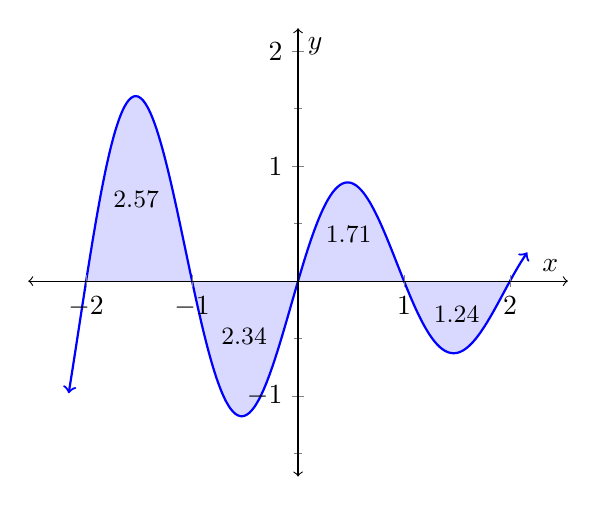
\begin{tikzpicture}
                \begin{axis}[grid=none, minor tick num=1,
                	axis x line=middle,
			xtick={
				-6.28318, -3.14159, 3.14159, 6.28318
			},
			xticklabels={
				$-2$, $-1$, $1$, $2$
			    },
                	xmax=8, xmin=-8,
                	axis y line=center,
                	ymax=2.2, ymin=-1.7,
	              	xlabel=$x$,ylabel=$y$, axis on top,
	              	axis line style = <->                    ]
                    \addplot[name path=f,smooth,domain=-6.8:6.8,color=blue,samples=100,thick,<->] {sin(deg(x))*exp(-0.1*x)};
		            \path[name path=axis] (axis cs:-8,0) -- (axis cs:8,0);
            
             \addplot+[blue!15] fill between[of=f and axis,soft clip={domain=-2*pi:2*pi}];

                    \node[label={90:{\small $2.57$}},inner sep=2pt] at (axis cs:-4.8,0.5) {};
                    \node[label={90:{\small $2.34$}},inner sep=2pt] at (axis cs:-1.6,-0.69) {};
                    \node[label={90:{\small $1.71$}},inner sep=2pt] at (axis cs:1.5,0.2) {};
                    \node[label={90:{\small $1.24$}},inner sep=2pt] at (axis cs:4.7,-0.5) {};
                \end{axis}
     1\end{tikzpicture}
     
\newpage

\Example Use the graph below to evaluate $\disp\int_{-2}^3 2x\, dx$.

\vspace{5mm}

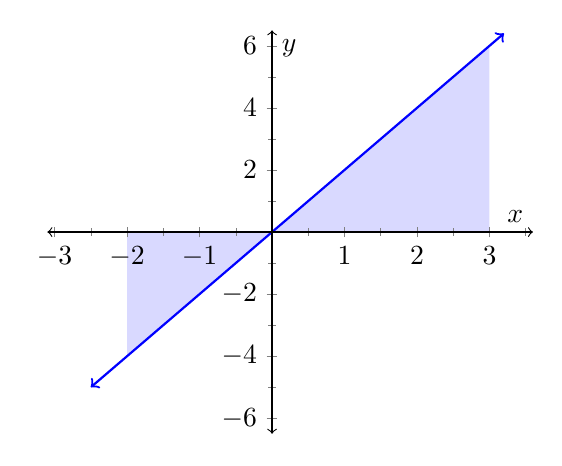
\begin{tikzpicture}[scale=0.9]
                \begin{axis}[grid=none, minor tick num=1,
                	axis x line=middle,
                	xmax=3.6, xmin=-3.1,
                	axis y line=center,
                	ymax=6.5, ymin=-6.5,
	              	xlabel=$x$,ylabel=$y$, axis on top,
	              	axis line style = <->                    ]
                    \addplot[name path=f,smooth,domain=-2.5:3.2,color=blue,samples=100,thick,<->] {2*x};
		            \path[name path=axis] (axis cs:-2,0) -- (axis cs:3.5,0);
            
             \addplot+[blue!15] fill between[of=f and axis,soft clip={domain=-2:0}];
             \addplot+[blue!15] fill between[of=f and axis,soft clip={domain=0:3}];
                \end{axis}
            \end{tikzpicture}
            
\vspace{3mm}

\Example Use the graph below to evaluate $\disp\int_{-1}^3\sqrt{4-(x-1)^2}\,dx$.

\vspace{5mm}

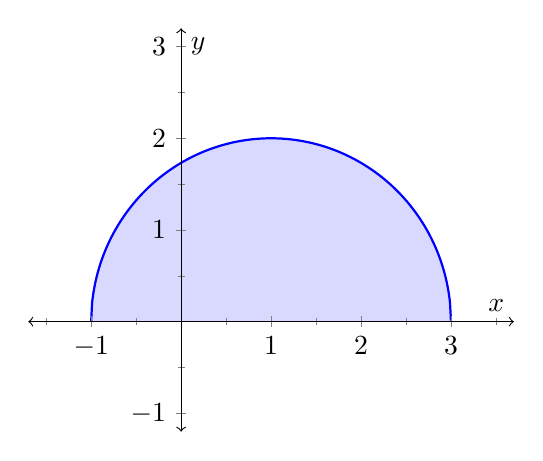
\begin{tikzpicture}[scale=.9]
                \begin{axis}[grid=none, minor tick num=1, 
                	axis x line=middle,
                	xmax=3.7, xmin=-1.7,
                	axis y line=center,
                	ymax=3.2, ymin=-1.2,
	              	xlabel=$x$,ylabel=$y$, axis on top,
	              	axis line style = <->                    ]
                    \addplot[name path=f,smooth,domain=-1:3,color=blue,samples=400,thick] {(4-(x-1)^2)^0.5};
		            \path[name path=axis] (axis cs:-3,0) -- (axis cs:3,0);
            
             \addplot+[blue!15] fill between[of=f and axis,soft clip={domain=-0.999:2.9999}];
                \end{axis}
            \end{tikzpicture}

\vspace{3mm}

\paragraph{Properties of the Definite Integral.}

\begin{itemize}
\item $\disp\int_a^b kf(x)\,dx=k\int_a^b f(x)\, dx$ for $k\in \R$
\item $\disp\int_a^b \big(f(x)\pm g(x)\big)\, dx=\int_a^b f(x)\,dx\pm\int_a^b g(x)\, dx$
\item $\disp\int_a^a f(x)\, dx=0$
\item $\disp\int_b^a f(x)\,dx=-\int_a^b f(x)\,dx$
\item $\disp\int_a^b f(x)\,dx=\int_a^c f(x)\,dx+\int_c^b f(x)\,dx$ where $c\in (a,b)$
\end{itemize}

\newpage

\Example Evaluate $\disp\int_0^1\big( f(x)-2g(x) \big)\,dx$ given that
$$\int_0^1 f(x)\,dx=e\text{ and }\int_1^0 g(x)\, dx=\pi.$$

\vspace{35mm}

\Example Use only the fact that $\disp\int_0^4 3x(4-x)\,dx=32$ and the properties of integrals to evaluate the following.
\begin{itemize}
	\item[\tc{1}] $\disp\int_4^0 3x(4-x)\,dx$
	
	\vspace{15mm}
	
	\item[\tc{2}] $\disp\int_0^4 x(x-4)\,dx$
	
	\vspace{15mm}
	
	\item[\tc{3}] $\disp\int_0^4 6x(4-x)\,dx$
	
	\vspace{15mm}
	
	\item[\tc{4}] $\disp\int_0^8 3x(4-x)\,dx$
	
	\vspace{15mm}
\end{itemize}

\newpage

\Example Use geometry and properties of integrals to evaluate
$$\int_0^1 \left( 2x+\sqrt{1-x^2}+1\right)\,dx.$$

\vspace{1mm}

Note: $\sqrt{1-x^2}$ represents an upper semicircle with $r=1$ centered at the origin.

\vspace{60mm}

\Example Evaluate the following definite integrals given the following.

$$\int_1^9 f(x)\,dx=-1\hspace{20mm}\int_7^9 f(x)\,dx=5\hspace{20mm}\int_7^9 h(x)\,dx=4$$

\begin{enumerate}
	\item[\tc{1}] $\disp\int_1^9 -2f(x)\,dx$
	
	\vspace{15mm}
	
	\item[\tc{2}] $\disp\int_7^9\big(2f(x)-3h(x)\big)\,dx$
	
	\vspace{15mm}
	
	\item[\tc{3}] $\disp\int_9^1 f(x)\,dx$
	
	\vspace{15mm}
	
	\item[\tc{4}] $\disp\int_9^7 \big( h(x)-f(x)\big)\,dx$
\end{enumerate}
\end{document}